\documentclass{article}

\usepackage[tiny]{titlesec}
\usepackage{pgfplots}
\usepackage{url}
\usepackage{graphicx}

\title{CSCI358 Assignment}
\author{Dilesh Mistry}

\graphicspath{ {images/} }
\setcounter{tocdepth}{1}

\begin{document}

\maketitle

\tableofcontents

\section[Banking]{You have been hired by a bank to help them harden their online banking service against phishing
attacks. Explain briefly the strengths and weaknesses of the following four possible countermeasures:
\\\\
In answering those questions you may need to explain how those countermeasures would be used.}

\subsection[SSL/TLS]{SSL/TLS client certificates issued to each customer.}

Advantages

- ensures that they will accessing your site and not someone else

Weakness

- very difficult to use/install as an end user
- there is a multitude of devices that it may need to be installed to

Usage

- you provide your TLS details to the client and if they try to go to a site it doesn't match, they will know quickly.

\subsection[Password Calculator]{A handheld password calculator issued to each customer}
Advantage

- its impossible to steal someone details without using the token
- even if they take the token password, it is unusable  

Weakness 

- they will need to have the password token on them to login to the site (something you have)
- if they lose it or replace they will lose access or someone else can login into their account  

Usage

- To login to a customer account they must use this password token

\subsection[Unique Picture]{Displaying a unique picture to each customer during the login process.}
Advantage

- a simple visual stimulus that is easy to use

Weakness 

- unless the picture changes, it can still be exploited
- what happens if the user cant see?

Usage

- After trying to login, there is a picture that appears that confirms that your are login into the bank


\subsection[Telephonic Second Factor]{Requiring that large payments, or payments to new recipients, be authorised by telephone or SMS as well as online.}
Advantage

- its impossible to a large emptying of bank account
- if a user wants to operate normally they only need to so a simple confirmation

Weakness 

- doesnt prevent for many small transactions
- doesnt increase security if it was small

Usage

- When a customer tries to do an transaction they will get a sms if its new or a large amount


\section{MachiavellianSoftwareEngineering}


\subsection[Waterfall Model]{What point is being made about the use of the waterfall model?}
It was the popular method at the time, even if the agile methods are better. 

\subsection[Prediction]{What tentative prediction is being made about the approach to software engineering in the future?}
People make choices that are simple but ill implemented. 

\subsection[Advantage]{What assurance related advantage does the article describe waterfall models as having? Explain your answer.}
It was easy to understand. 

This allow people who were properly implement it and understand what is happening. 

\section[ALE Table]{For the following information draw up an ALE table and make a recommendation on the basis of it: let $E_{i}, 1 \le i \le 10$ be the events that could cause damage. Let the respective frequency of events be ${1.4, 3, 0.2, 5, 150, 0.04, 0.5, 1, 6, 0.0001}$ and the respective cost per event be ${4, 9, 30, 7, 0.5, 700, 60, 30, 0.5, 1600}$.}


\begin{tabular}{c|c|c|c}
\hline
Loss Event & Frequency & Cost Per Event & Expected Costs \\
1 & 1.4 & 3 & 4.2\\
2 & 3 & 9 & 27\\
3 & 0.2 & 30 & 6 \\
4 & 5 & 7 & 35\\
5 & 150 & 0.5 & 75\\
6 & 0.04 & 700 & 28\\
7 & 0.5 & 60 & 30\\
8 & 1 & 30 & 30\\
9 & 6 & 0.5 & 3\\
10 & 0.0001 & 1600 & 0.16\\
\end{tabular}


\section[Context and Information]{Give an example of how context affects the way we interpret information. Don’t use something
mentioned in the lectures or lecture notes.}

The phrase "I want strong security" comes to mind.

When a home-owner wants security if it just a person trying to protect they family home, an alarm system, with a couple of cameras is sufficient. However, if the home-owner is trying to store money in their house and maybe have sensitive information then an alarm system is not enough, and you might need to start thinking about safe, infra red camera, security staff. 

You cant just state that you want "strong security" without giving context of the application. 


\section[Risk Thermostat]{What role does the ”risk thermostat” play in determining the likely effect of introducing a security control?}

A risk thermostat \cite{riskthermo} is basically a model which takes in account the various factors that a entity can take when making a choice. The risk thermostat model, dictates if you are a person who 

\begin{itemize}
\item takes risks
\item has little losses
\end{itemize}

You will be likely to implement a security control which takes into account all the risks, since your risk thermostat is high.

However if you are person who 

\begin{itemize}
\item doesn't takes risks
\item is very likely to take a loss
\end{itemize}

Then you will be more likely implement a security control that takes into account more aspects of risk, since you are low on risk thermostat. 

\section[Hill Climbing]{These questions relate to hill climbing attacks. This has very little to do with the ”climbing the mountain” exercise in the lectures:}

\subsection[Hill Climbing and biometrics]{Explain how a hill climbing attack works in the context of biometrics.}

You try to use a feedback loop between the system and you to try to successively get more accurate with your attacks until you are able to gain access. 

\subsection[Hill Climbing Assumptions]{What assumptions underlay the use of this attack?}

You are able to repetitively, (and some aspect of automation) attempt access to the system without interruption. 

\subsection[Hill Climbing and presentation]{Based on the assumptions, how might we provide protection against a hill climbing attack?}

\begin{itemize}
\item Prevent automation of repeated failed attempts.
\item Have some form of second factor of authentication. 
\end{itemize}

\section[Buying Cars]{Consider that number of people N willing to buy cars at a given price P varies according to the
function. \[N=5000-2P\] \\
Note that, for example, a person willing to buy a car at a price of \$200 will also be willing to buy a car at \$100 and will be included under both. This is not a function of the number of persons with the price returned as the most they will pay}

\subsection[Graph]{Provide a graph of N vs P, in an appropriate range, with N on the x axis and P on the y axis.
Be sure to appropriately label the intercepts}

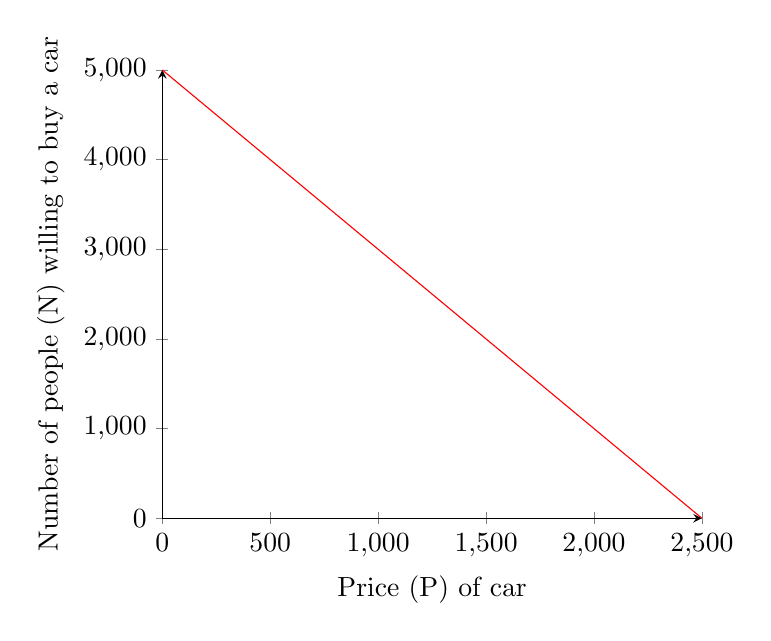
\begin{tikzpicture}
\begin{axis}[
    axis lines = left,
    xlabel = Price (P) of car,
    ylabel = Number of people (N) willing to buy a car,
]
%Below the red parabola is defined
\addplot [
    domain=0:2500, 
    samples=100, 
    color=red,
]
{5000 - 2*x};
\end{axis}
\end{tikzpicture}

\subsection[competitive]{Assume we have a competitive marketplace with a total of 200 cars for sale. How much money
will be spent on purchasing cars? Justify your answer.}

\begin{eqnarray*}
N&=&5000-2*P \\
200&=&5000-2*P \\
P&=&2400 \\
\end{eqnarray*}
That is a cost per car. However then there is 200 cars so \\
\begin{eqnarray*}
TotalGains&=& N*P \\
&=& 200 * 2400 \\
&=& 480000 \\
\end{eqnarray*}

\subsection[monopoly]{Now assume we instead have a monopoly. You still have 200 cars for sale. You are only allowed
to sell cars at four different prices and you must sell fifty cars at each price. What is the most
you can make from car sales? Justify your answer.}

For first 50 cars the cost is 
\begin{eqnarray*}
N&=&5000-2*P_1 \\
200&=&5000-2*P_1 \\
P_1&=&2400 \\
\end{eqnarray*}

For next 50 cars the cost is
\begin{eqnarray*}
N&=&5000-2*P_2 \\
150&=&5000-2*P_2 \\
P_2&=&2425 \\
\end{eqnarray*}

For next 50 cars the cost is
\begin{eqnarray*}
N&=&5000-2*P_3 \\
100&=&5000-2*P_3 \\
P_3&=&2450 \\
\end{eqnarray*}

For next 50 cars the cost is
\begin{eqnarray*}
N&=&5000-2*P_4 \\
50&=&5000-2*P_4 \\
P_4&=&2475 \\
\end{eqnarray*}

Then the total gains are

\[50*P_1 + 50*P_2 + 50*P_3 + 50*P_4\]
\[50*2400 + 50*2425 + 50*2450 + 50*2475\]
\[487500\]


\section[Dilbert]{Consider the Dilbert cartoons listed below. Briefly explain what concept each relates to in the
context of CSCI358. There may be more than one acceptable answer. Justify your answer.}
\subsection{01-Feb-1994}
\includegraphics[scale=0.7]{01-Feb-1994}

The software developer is adding more risk than he needed to by adding bad conventions for shortcuts, and allowing them to edit source code. 
\subsection{29-Jan-2010}
\includegraphics[scale=0.7]{29-Jan-2010}

This works in a similar manner of phishing. Deceiving the target to leverage something. 
\subsection{31-Dec-2002}
\includegraphics[scale=0.7]{31-Dec-2002}

Biometrics has obvious downside, that being that if a person lacks the ability to do a task, such as eye verification after eye surgery, they will not be able to enter the system even if they are valid. 
\subsection{01-Feb-2011}
\includegraphics[scale=0.7]{01-Feb-2011}

Other sectors of the business only wants to understand the technical requirements in context 
\section[Laws]{Describe Moore’s Law, Dennard Scaling and Amdahl’s Law}

Moores Law -  Over the history of computing hardware, the number of transistors in a dense integrated circuit doubles approximately every two years. \cite{moores}

Dennard Scaling - That as transistors get smaller their power density stays constant, so that the power use stays in proportion with area: both voltage and current scale (downward) with length. \cite{dennard}

Amdahl Law - Is used to find the maximum expected improvement to an overall system when only part of the system is improved. \cite{amdahl}

\section[Computational Speed]{Explain the relationships between the three concepts above and the ramifications for computational
speed.}

As time goes on due to Moores Law and dennard scaling, we will have more powerful and denser chips, however due to Amdahl law, we should understand that this will bring advantage in a only part of the system. So even though we are getting chips, we need to consider the whole system when determining computational speed. 

\section[Asset]{Consider that I have an asset worth \$2000. There are two independent threats. The first occurs with probability 0.05 and would reduce the value of the asset to \$100, while the second occurs with probability 0.01 and would completely destroy the asset. Both could occur. What would be the threshold value at which buying insurance would be ”worthwhile for both parties”? Be sure to show working. }

\begin{eqnarray*}
2000*0.05 + x*0.95 + insure &=& 100 + 1900 + insure \\
x*0.95 &=& 1900 \\
x &=& 2000 \\
\end{eqnarray*}

In the first case you would want to pay around \$2000.

\begin{eqnarray*}
2000*0.01 + x*0.99 + insure &=& 0 + 2000 + insure \\
x*0.99 &=& 2000 \\
x &=& 2,020.20 \\
\end{eqnarray*}

You would want to pay \$2020.20
\section[Online Gaming]{Describe a real example of an attack against a on-line gaming system. Find out how the problem was dealt with.}
Scamming logins with keyboards loggers. My MMO introduced a random keypad pin that you must use to login. The keys on the virtual keypad are randomly placed. 

\section[Fault Injection]{Describe how you could use fault injection in the context of plagiarism detection.}
I would use fault injection by having texts that i know are similar but semantically different. Also i would try to test for synonyms. 


\section[anonymity terminology]{ Describe the following termininology in the content of anonymity:}

\subsection{Anonymity}
Being unable to identity an entity in a system. 

\subsection{Unlinkability}

There is no way to link a instance to a person
\subsection{Unobservability}

You aren't able to observe a status of an entity

\subsection{Pseudonymity}

You are allowed to use a pseudonym. 

\section[ALE Table]{Complete the following ALE table. Explain what each row/column represents, and indicate units for entries. Explain what actions this specific table suggests we should take.}

\begin{tabular}{c|c|c|c}
\hline
Loss Event &  Cost Per Event (\$) & Frequency  & Expected Costs (\$) \\
A & 20000 & 0.1 & 200\\
B & 18000 & 0.5 & 9000\\
C & 3000 & 0.333 & 1000 \\
D & 550 & 2 & 1100\\
E & 25 & 4 & 100\\
F & 10 & $\ge$ 4 & $\ge$ 40\\
\end{tabular}

Row - An event

Column - 

\begin{itemize}
\item Loss Event

What event
\item Cost per event
What the cost if the event is trigged
\item Frequency

The number of time an event will occur

\item Expected Costs

How much are you expected to lose over a time period
\end{itemize}

\section[Code Of Conduct]{The next few questions relate to the \texttt{Australian Computer Society Code of Professional Conduct and Professional Practice}, which can be found in \texttt{CodeofProfConductPractice.pdf}}.

\subsection{Describe the meaning of the redundancy referred to in the Code. How does it differ to the redundancy in the context of this subject and where in the code does that meaning relate to?}


\begin{quote}
Ensure that there are adequate procedures available to delete erroneous, redundant 
and out of date data from files. 
\end{quote}

In the code, redundancy is related to it in development, however in this subject we use redundancy as a term for having multiple systems for a single task. 

\subsection{The term \texttt{integrity} is used in several ways inside the Code. Describe each of the uses of the term in the Code.}

\begin{itemize}
\item In terms of professional conduct
\begin{quote}
Do not breach public trust in the profession or the specific trust of your clients and 
employers 
\end{quote}
\item Security

Ensuring that whatever we do, that the integrity of the data is always held true. 

\end{itemize}

\subsection{Describe how assurance, in the sense of Anderson’s framework, fits within the Code}

As a member of the Australian Computer Society we can assure others that we will operate under this code. We provide an insurance of minimal operating standards. 

\section[Redundant Systems]{These questions relate to diversity in redundant systems:}

\subsection{What does diversity mean in the context of redundant systems?}

Having multiple and different implementations of a system. 

\subsection{Why does diversity in redundant systems matter?}

It is useful since if one system fails there is another backup system that the issue might not exist. 

For example when openssl bug was found, people could have also been using polarssl as well as an alternative library. 

\begin{thebibliography}{9}
\bibitem{riskthermo} The Risk of Freedom: individual liberty and the modern world, Institute of United States
Studies, 1999 
\bibitem{moores} Moore, Gordon E. (1965). "Cramming more components onto integrated circuits". Electronics Magazine. p. 4.
\bibitem{dennard} Dennard, Robert H.; Gaensslen, Fritz; Yu, Hwa-Nien; Rideout, Leo; Bassous, Ernest; LeBlanc, Andre (October 1974). "Design of ion-implanted MOSFET's with very small physical dimensions". IEEE Journal of Solid State Circuits SC–9 (5).
\bibitem{amdahl} Rodgers, David P. (June 1985). "Improvements in multiprocessor system design". ACM SIGARCH Computer Architecture News archive (New York, NY, USA: ACM) 13 (3): 225–231.
\bibitem{Anon_Terminology} \url{http://dud.inf.tu-dresden.de/literatur/Anon_Terminology_v0.34.pdf}
\end{thebibliography}
\end{document}
